\chapter{Des algorithmes complexes...}
\section{Optimisation théorique des méthodes}
\subsection{Préconditionnement pour une méthode itérative}

On peut illustrer les problèmes des méthodes itératives à travers la méthode du gradient conjugué. En effet, les conditionnements des matrices étudiées sont parfois très grands et il est ainsi nécessaire d'effectuer une opération dite de préconditionnement afin de minimiser les résidus des itérations.\\

Dans ce but, on introduit une matrice de préconditionnement que l'on note $C$. Cette matrice interviendra dans l'algorithme du gradient conjugué afin de l'optimiser. La matrice $C$ diffèrera selon la méthode de préconditionnement choisie. Dans ce mémoire, nous nous focaliserons sur la méthode SSOR. \\

L'objectif mathématique de l'introduction de la matrice $C$ est de mieux répartir les valeurs propres du système linéaire étudié, ce qui va permettre d'accélérer la méthode du gradient conjugué. \\

En effet, une meilleure répartition des valeurs propres de la matrice liée au système étudié permet de faire rapprocher les lignes de niveau de la fonction associée au système vers des cercles. Cela permettra ensuite d'avoir moins d'itérations pour la méthode de descente du gradient conjugué.\\

Nous aborderons dans ce mémoire, deux méthode de préconditionnement, celle de Jacobi et celle dite SSOR. Les méthodes de préconditionnement du gradient conjugué introduisent une suite $z_k$, résultant du produit matriciel entre $C$ et le résidu à l'ordre $k$, noté $r_k$. Ensuite, les calculs des coefficients nécessaires à l'application de la méthode utiliseront à la fois la suite $z_k$ et le résidu $r_k$. 
\subsubsection{Préconditionnement de Jacobi}
Le préconditionnement de Jacobi est le plus simple pour le gradient conjugué. Cette méthode est donc intéressante lorsqu'une grande précision n'est pas requise. Étant moins précise, elle est plus facile à  implémenter numériquement mais n'améliore pas autant la résolution du problème par méthode du gradient conjugué que la SSOR par exemple.\\

Le préconditionnement de Jacobi consiste à prendre pour matrice de pré-\\conditionnement $C$ :
$$
C_{i,j}
\begin{cases}
A_{i,i}\text{ si } i=j\\
0 \text{ sinon}
\end{cases}
$$

La matrice $C$ correspond donc à la diagonale de $A$. Le produit entre $C$ et le résidu se fait aisément puisque tous les termes extradiagonaux sont nuls. Cependant, si l'on souhaite avoir une méthode de préconditionnement améliorant grandement les performances de l'algorithme du gradient conjugué, le préconditionnement de Jacobi n'est pas adapté. Pour ces cas de figure, nous pouvons utiliser la méthode SSOR.
\subsubsection{Préconditionnement SSOR}
La méthode SSOR (Symetric Successive Over Relaxation) permet d'améliorer le gradient conjugué de meilleure manière que la méthode de Jacobi mais elle est plus difficile à mettre en place. En effet, la matrice $A$ du système $Ax=b$ doit être symétrique.\\

Une méthode simple de décrire cette méthode est de la présenter comme étant deux applications de la méthode SOR (décrite auparavant), successives, dans des sens contraires. La première application permet de préconditionner le système et la deuxième permet de le résoudre.\\

Concrètement, on décompose la matrice $A$ en :
$$
A=L+D+L^T
$$
$D$ étant la matrice comportant la diagonale de $A$ et $L$ une matrice triangulaire inférieure. La matrice $C$ est donc définie par :
$$
C(\omega)=\frac{\omega}{2-\omega}(\frac{D}{\omega}+L)D^{-1}(\frac{D}{\omega}+L^T)
$$

Étant donné que cette méthode consiste en deux SOR successives, la condition nécessaire et suffisante de convergence de la méthode est identique à celle de la SOR. Il suffit que le paramètre de relaxation $\omega$ soit dans l'intervalle $]0;2[$.\\

\subsection{Les limites de l'optimisation mathématique}

Bien que les méthodes d'optimisation numérique vues précédemment permettent d'améliorer de manière significative les performances d'un algorithme (plus particulièrement celui du gradient conjugué dans le cas précédent), cela peut ne pas être suffisant lorsque nous avons affaire à des systèmes de grande taille avec des coefficients élevés dans la matrice liée au système. Il est donc nécessaire de coupler l'optimisation mathématique (par les méthodes de préconditionnement), à des études de performances numériques avec des méthodes d'optimisation lors de l'implémentation de ces algorithmes sur nos machines.

\newpage
\section{Étude des performances}

\subsection{Implémentation}
% -> pourquoi C++ ?
\subsubsection{Pourquoi C++ ?}
Au premier abord, une implémentation optimisée doit être écrite pour une plateforme en particulier, en utilisant le langage de programation de plus bas niveau afin de s'approcher au mieux de la réalité du matériel. Réalistiquement, une telle approche est coûteuse en temps de développement et en temps de documentation afin de comprendre réellement l'architecture et le set d'instructions. \\

La meilleure solution est alors de s'abstraire d'une couche et d'adopter un langage tel que le C, le C++, le Fortran ou le Rust. Le choix est alors au développeur, est ici le langage C++ a fait l'objet de notre choix.\\



%-> indicateurs de performance
\subsubsection{Indicateurs de performance}
Afin de mesurer au mieux nos algorithmes, on peut se demander - à raison - quels indicateurs sont les plus cohérents afin de comparer leurs performances. Un choix se présente alors à nous : quelle dimension mesurer ? Les dimensions mesurées couramment sont celles de la vitesse d'éxécution et l'utilisation mémoire. Nous avons ici choisi de nous tourner vers les mesures de vitesse , mais là encore une multitude d'indicateurs sont à notre disposition : temps d'éxécution, nombre de cycles, nombre de branches, requêtes au cache, etc...\\

Afin de faire un choix pertinent, nous nous sommes tournés vers les experts du site StackOverflow.com (voir question : \url{https://stackoverflow.com/questions/55650592}). La réponse de Peter Cordes, dont la réputation sur le site est de plus de 135000, et qui est une référence pour les questions d'optimisation, nous a répondu :\\

\begin{quote}
	Time is the most relevant indicator.\\
	This is why most profilers default to measuring / sampling time or core clock cycles. Understanding where your code spends its time is an essential first step to looking for speedups. First find out what's slow, then find out why it's slow.
\end{quote}


%-> problèmes rencontrés (PLU, déterminant, lstsqr)
\subsubsection{Problèmes rencontrés}
En C++, les bibliothèques d'algèbre linéaire globalement disponibles ont plusieurs désavantages :
\begin{itemize}
	\item grande complexité
	\item temps de compilation souvent très grand (compté en heures)
	\item difficulté d'accès
\end{itemize}

Ces points, ajoutés à notre besoin d'apprentissage et d'expérience, nous ont mené à choisir d'implémenter par nous-mêmes l'ensemble des fonctionnalités dont nous aurons besoin pour implémenter les différents algorithmes.\\

L'implémentation des opérations basiques sur les matrices (multiplication, somme, transposée, extraction d'une diagonale, génération aléatoire, rang, etc...) a posé un ensemble de problèmes qui n'avait pas été anticipé, donc une charge de travail plus grande que prévu. Par exemple, la vérification des résultats des différents algorithmes est faite en cherchant la matrice inverse de A : $A^{-1}$ qui doit être trouvée grâce à une décomposition PLU et non par une implémentation naïve $A^{-1} = \frac{1}{det(1)} * comatrice(A)^{T}$ qui, à cause de sa complexité en $n!$, impose une charge processeur bien trop grande.

% LSTSQR
Après avoir implémenté toutes les bases, il nous a fallu implémenter les différents algorithmes étudiés : Jacobi, Gauss-Seidel, Richardson (non-mesuré car redondant avec les méthodes précédentes), SOR, GMRES. En particulier, une difficulté s'est posée lors de l'implémentation de l'algorithme GMRES, celui-ci nécessitant une minimisation des moindres carrés en dimension N. Il nous a fallu nous tourner vers une bibliothèque externe, ne connaissant - pour l'instant - pas les méthodes de résolution adaptées.

%-> méthode de mesure 
\subsubsection{Méthode de mesure}
Les processeurs actuelles disposent d'une horloge de haute précision, basée sur le nombre de cycles d'horloge écoulés. Celle-ci est fiable à la nanoseconde près, et c'est donc celle-ci que nous avons choisi d'utiliser afin de garantir une bonne précision. Le code suivant permet la mesure en utilisant l'horloge la plus précise que le système peut supporter :

\begin{minted}{cpp}
	//START TIME MEASUREMENT
	auto begin(std::chrono::high_resolution_clock::now());
	
	// CALL FUNCTION
	std::tuple<Matrix<T>, Matrix<T>, Matrix<T>> res0(gaussSeidel(A));
	std::tuple<Matrix<T>, long long, T> result(
		iter_generale(std::get<1>(res0), std::get<2>(res0), b, x0, curprec, (long long)1e9)
	);
	
	// END TIME MEASUREMENT
	auto end(std::chrono::high_resolution_clock::now());
	auto duration(std::chrono::duration_cast<std::chrono::nanoseconds>(end - begin).count());

\end{minted}

Il faut noter dans le code précédent, les variables de type automatique $begin$ et $end$ sont en pratique des instances de $std::time\_point$. Les fonction utilisées pour la mesure de temps sont définies dans $<chrono>$.\\



\subsection{Analyse des mesures}


Nous avons souhaité comparer les différents algorithmes en faisant varier un certain nombre de paramètres, notamment la précision souhaitée et la taille des matrices. Dans les graphiques ci-dessous, l'ensemble des points de mesure que nous allons étudier sont représentés.


%-> graphes 3D
\begin{figure}[H]
	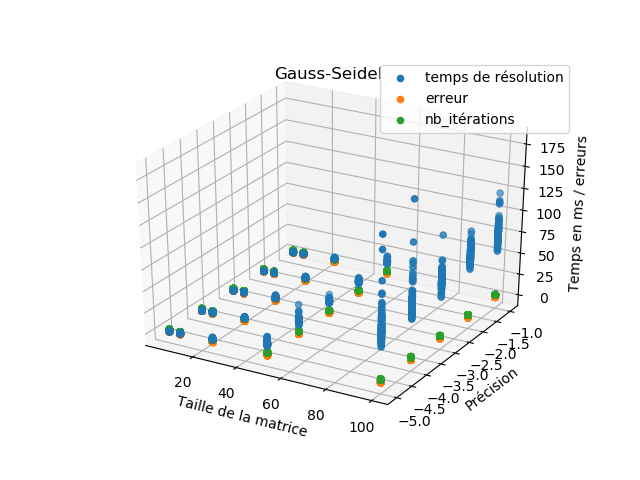
\includegraphics{../codes/Data/gauss-seidel3D.png}
	\caption{Représentation graphique tridimensionnelle des performances de l'algorithme de Gauss-Seidel}
\end{figure}

\begin{figure}[H]
	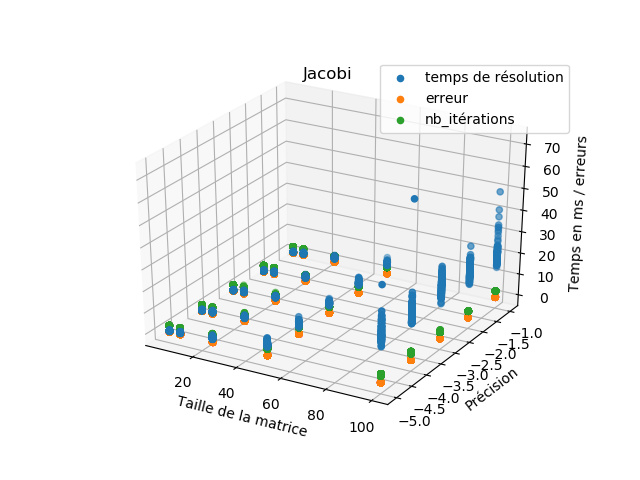
\includegraphics{../codes/Data/jacobi3D.png}
	\caption{Représentation graphique tridimensionnelle des performances de l'algorithme de Jacobi}
\end{figure}

\begin{figure}[H]
	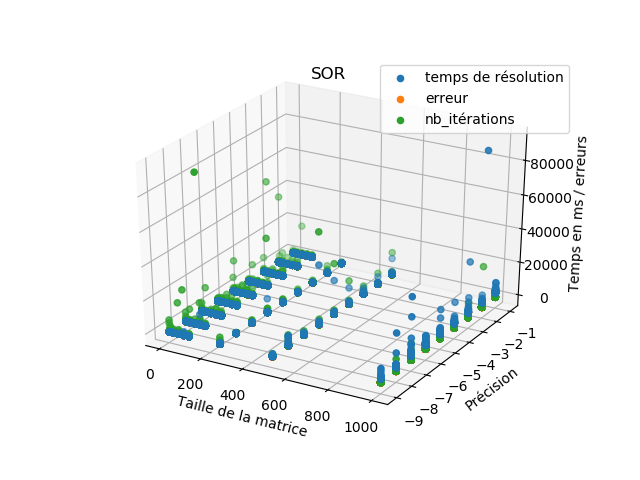
\includegraphics{../codes/Data/sor3D.png}
	\caption{Représentation graphique tridimensionnelle des performances de l'algorithme SOR}
\end{figure}

\begin{figure}[H]
	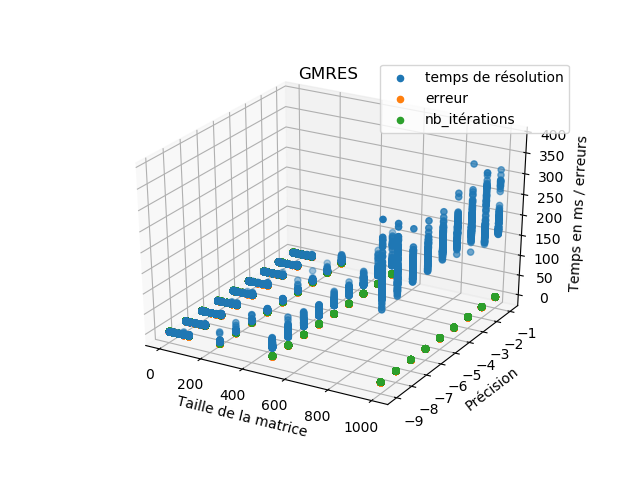
\includegraphics{../codes/Data/gmres.png}
	\caption{Représentation graphique tridimensionnelle des performances de l'algorithme GMRES}
\end{figure}

Les performances de la méthode GMRES pour une précision $\epsilon = 10^{-15}$ sont représentés ci-dessous.
%-> graphes 2D


%-> analyse des mesures
% 1. Précision ne change pas grand chose
% 2. Augmentation du temps de calcul en fonction de la taille
% 3. itération à 1 pour GMRES
% 4. évolution des erreurs


%-> conclusion

\subsection{Ouverture et discussion}
\subsubsection{Optimisation numérique}
%-> Optimisation encore possible + comment faire
Un certain nombre d'optimisations n'ont pas été mises en place dans le code C++, notamment à cause d'un manque de ressources temporelles. Les performances des algorithmes ont probablement encore une marge de progression en terme de performances située entre 5 et 10 fois la vitesse actuelle, ceci étant lié à une possible réduction du nombre de copies de matrices effectuées, une optimisation des lignes d'exécution sur les boucles critiques (i.e dans lesquelles le processeur passe le plus de temps), et une meilleure gestion du parallélisme.


\subsubsection{méthode des moindres carrés}
%-> least squares
L'implémentation de l'algorithme nécessitant de résoudre un problème des moindres carrés, nous avons fait le choix de faire appel à une bibliothèque externe. Celle-ci ajoute considérablement au temps d'exécution, de par le besoin de copie de données (structure de données différente), et malgré cela, la méthode GMRES est largement supérieure en terme de performances. Une implémentation par nos soins d'un algorithme tel que L-BFGS, OWL-QN (quasi-Newton) ou autres pourrait encore diviser le temps mesuré.


\subsubsection{mesure}
%-> Variance induite par CPU et solution
Le simple fait d'exécuter ce test sur un PC muni d'un système d'exploitation impose une variance sur nos mesures, celui-ci étant en mesure d'interrompre notre programme au profit d'un processus d'importance supérieure à tout moment. C'est pourquoi il nous a fallu prendre un échantillon de 100 mesures par combinaison d'algorithme, de précision et de taille de matrices.\\

Il est possible de s'abstraire de ce système d'exploitation et d'améliorer drastiquement la précision des mesures en compilant pour un système embarqué, qui lui n'est pas muni d'un système d'exploitation et est en mesure de compter exactement le nombre de cycles écoulés (exemple: architecture AVR d'Atmel). Les mesures seraient alors entièrement reproductibles et sans variance, en admettant une génération aléatoire reproductible grâce à une méthode d'initialisation des algorithmes connue (seed). 


